\documentclass[11pt,a4paper,twocolumn]{article}
\usepackage[english,greek]{babel}
\usepackage[utf8]{inputenc}
\usepackage{nimbusserif}
\usepackage[T1]{fontenc}
\usepackage[left=1.50cm, right=1.50cm, top=2.00cm, bottom=2.00cm]{geometry}
\usepackage{amsmath}
\let\myBbbk\Bbbk
\let\Bbbk\relax
\usepackage[amsbb,subscriptcorrection,zswash,mtpcal,mtphrb,mtpfrak]{mtpro2}
\usepackage{graphicx,multicol,multirow,enumitem,tabularx,mathimatika,gensymb,venndiagram,hhline,longtable,tkz-euclide,fontawesome5,eurosym,tcolorbox,tabularray}
\usepackage[explicit]{titlesec}
\tcbuselibrary{skins,theorems,breakable}
\newlist{rlist}{enumerate}{3}
\setlist[rlist]{itemsep=0mm,label=\roman*.}
\newlist{alist}{enumerate}{3}
\setlist[alist]{itemsep=0mm,label=\alph*.}
\newlist{balist}{enumerate}{3}
\setlist[balist]{itemsep=0mm,label=\bf\alph*.}
\newlist{Alist}{enumerate}{3}
\setlist[Alist]{itemsep=0mm,label=\Alph*.}
\newlist{bAlist}{enumerate}{3}
\setlist[bAlist]{itemsep=0mm,label=\bf\Alph*.}
\newlist{askhseis}{enumerate}{3}
\setlist[askhseis]{label={\Large\thesection}.\arabic*.}
\renewcommand{\textstigma}{\textsigma\texttau}
\newlist{thema}{enumerate}{3}
\setlist[thema]{label=\bf\large{ΘΕΜΑ \textcolor{black}{\Alph*}},itemsep=0mm,leftmargin=0cm,itemindent=18mm}
\newlist{erwthma}{enumerate}{3}
\setlist[erwthma]{label=\bf{\large{\textcolor{black}{\Alph{themai}.\arabic*}}},itemsep=0mm,leftmargin=0.8cm}

\newcommand{\kerkissans}[1]{{\fontfamily{maksf}\selectfont \textbf{#1}}}
\renewcommand{\textdexiakeraia}{}

\usepackage[
backend=biber,
style=alphabetic,
sorting=ynt
]{biblatex}

\DeclareTblrTemplate{caption}{nocaptemplate}{}
\DeclareTblrTemplate{capcont}{nocaptemplate}{}
\DeclareTblrTemplate{contfoot}{nocaptemplate}{}
\NewTblrTheme{mytabletheme}{
\SetTblrTemplate{caption}{nocaptemplate}{}
\SetTblrTemplate{capcont}{nocaptemplate}{}
\SetTblrTemplate{contfoot}{nocaptemplate}{}
}

\NewTblrEnviron{mytblr}
\SetTblrStyle{firsthead}{font=\bfseries}
\SetTblrStyle{firstfoot}{fg=red2}
\SetTblrOuter[mytblr]{theme=mytabletheme}
\SetTblrInner[mytblr]{
rowspec={t{7mm}},columns = {c},
width = 0.85\linewidth,
row{odd} = {bg=red9,fg=black,ht=8mm},
row{even} = {bg=red7,fg=black,ht=8mm},
hlines={white},vlines={white},
row{1} = {bg=red4, fg=white, font=\bfseries\fontfamily{maksf}},rowhead = 1,
hline{2} = {.7mm}, % midrule  
}
\newcounter{askhsh}
\setcounter{askhsh}{1}
\newcommand{\askhsh}{\large\theaskhsh.\ \addtocounter{askhsh}{1}}

\titleformat{\section}{\Large}{\kerkissans{\thesection}}{10pt}{\Large\kerkissans{#1}}

\setlength{\columnsep}{5mm}
\titleformat{\paragraph}
{\large}%
{}{0em}%
{\textcolor{red!80!black}{\faSquare\ \ \kerkissans{\bmath{#1}}}}
\setlength{\parindent}{0pt}

\newcommand{\eng}[1]{\selectlanguage{english}#1\selectlanguage{greek}}

\newcommand{\roloi}[4][]{
\draw[line width=.5mm,#1] (0,0) circle(2);
\foreach \n in {1,2,...,12}{
\tkzDefPoint(30*\n-90:2){A_\n}
%\tkzDrawPoint(A_\n)
\node at (-30*\n+90:1.65){\n};}
\draw[plm,,#1] (0,0)--(90-30*#2-0.5*#3:1);
\draw[pl,#1] (0,0)--(90-6*#3-0.1*#4:1.5);
\draw[#1](0,0)--(90-6*#4:1.2);
\tkzDrawPoint[fill=#1,color=#1](0,0)
\foreach \s in {1,2,...,12}{
\draw[#1](90-30*\s:1.85)--(90-30*\s:2);}
\foreach \t in {1,2,...,60}{
\draw[#1](90-6*\t:1.93)--(90-6*\t:2);}}

\begin{document}
\twocolumn[{
\centering
\kerkissans{{\huge Η έννοια του τριγωνομετρικού αριθμού}\\\vspace{3mm} {\Large ΑΣΚΗΣΕΙΣ}}\vspace{5mm}}]
\paragraph{Τριγωνομετρικοί αριθμοί σε τρίγωνο}
\askhsh
Να υπολογίσετε τους τριγωνομετρικούς αριθμούς της γωνίας $ \omega $ σε καθένα από τα παρακάτω ορθογώνια τρίγωνα.
\begin{multicols}{2}
\begin{alist}
\item\tikzitem 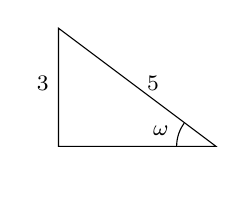
\begin{tikzpicture}
\draw (-1,0.5) -- (-1,-1) -- (1,-1) -- cycle;
\draw (0.5955,-0.7061) arc (143.9987:180:0.5);
\node at (0.3,-0.8) {\footnotesize$\omega$};
\node at (-1.2,-0.2) {\footnotesize$3$};
\node at (0.2,-0.2) {\footnotesize$5$};
\node at (-0.1,-1.2) {\footnotesize$  $};
\end{tikzpicture}
\item\tikzitem 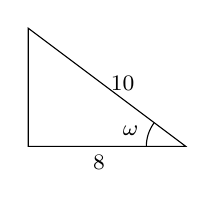
\begin{tikzpicture}
\draw (-1,0.5) -- (-1,-1) -- (1,-1) -- cycle;
\draw (0.5955,-0.7061) arc (143.9987:180:0.5);
\node at (0.3,-0.8) {\footnotesize$\omega$};
\node at (-0.1,-1.2) {\footnotesize$8$};
\node at (0.2,-0.2) {\footnotesize$10$};
\end{tikzpicture}
\item\tikzitem 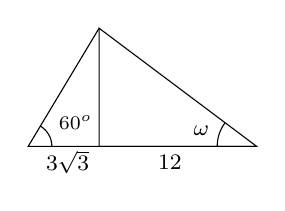
\begin{tikzpicture}
\draw (-1,0.5) -- (-1,-1)  -- (1,-1) -- cycle;
\draw (0.5955,-0.7061) arc (143.9987:180:0.5);
\node at (0.3,-0.8) {\footnotesize$\omega$};
\node at (-0.1,-1.2) {\footnotesize$12$};
\draw (-1,0.5) -- (-1.9,-1) -- (1,-1);
\draw (-1.6,-1) arc (0:57.9421:0.3);
\node at (-1.3,-0.7) {\scriptsize$60^o$};
\node at (-1.4,-1.2) {\footnotesize$3\sqrt{3}$};
\end{tikzpicture}
\item\tikzitem 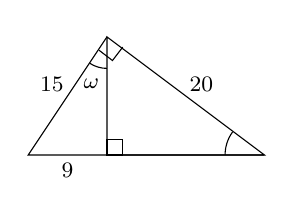
\begin{tikzpicture}
\draw (-1,0.5) -- (-1,-1)  -- (1,-1) -- cycle;
\draw (0.5955,-0.7061) arc (143.9987:180:0.5);
\node at (-1.2,-0.1) {\footnotesize$\omega$};
\node at (0.2,-0.1) {\footnotesize$20$};
\draw (-1,0.5) node (v1) {} -- (-2,-1) -- (1,-1);
\node at (-1.7,-0.1) {\footnotesize$15$};
\draw (-1,0.1) arc (-90:-123:0.4);
\draw (-1.1,0.33) -- (-0.93,0.2) -- (-0.8,0.37);
\draw  (-1,-0.8) rectangle (-0.8,-1);
\node at (-1.5,-1.2) {\footnotesize$9$};
\end{tikzpicture}
\end{alist}
\end{multicols}
\paragraph{Μοίρες - Ακτίνια}
\askhsh
Οι παρακάτω γωνίες οι οποίες είναι δοσμένες σε μοίρες να εκφραστούν σε ακτίνια (\eng{rad}).
\begin{multicols}{3}
\begin{alist}
\item $ 30\degree $
\item $ 60\degree $
\item $ 45\degree $
\item $ 120\degree $
\item $ 150\degree $
\item $ 300\degree $
\item $ 270\degree $
\item $ 240\degree $
\item $ 330\degree $
\item $ 400\degree $
\item $ 480\degree $
\item $ 1200\degree $
\end{alist}
\end{multicols}
\askhsh
Οι παρακάτω γωνίες οι οποίες είναι δοσμένες σε ακτίνια να εκφραστούν σε μοίρες.
\begin{multicols}{3}
\begin{alist}
\item $ \frac{\pi}{4} $
\item $ \frac{2\pi}{3} $
\item $ \frac{\pi}{6} $
\item $ \frac{3\pi}{4} $
\item $ \frac{2\pi}{5} $
\item $ \pi $
\item $ \frac{3\pi}{2} $
\item $ \frac{4\pi}{5} $
\item $ 24\pi $
\item $ \frac{35\pi}{3} $
\item $ \frac{105\pi}{4} $
\item $ 400\pi $
\end{alist}
\end{multicols}
\paragraph{Τριγωνομετρικοί αριθμοί}
\askhsh
Να υπολογίσετε τους τριγωνομετρικούς αριθμούς των παρακάτω γωνιών.
\begin{multicols}{3}
\begin{alist}
\item $ 390\degree $
\item $ 450\degree $
\item $ 780\degree $
\item $ 1260\degree $
\item $ 1125\degree $
\item $ 1845\degree $
\end{alist}
\end{multicols}
\askhsh
Να υπολογίσετε τους τριγωνομετρικούς αριθμούς της γωνίας $ x\hat{O}M $ η οποία σχηματίζεται μέσα σε ένα ορθοκανονικό σύστημα συντεταγμένων $ xOy $ για καθένα από τα παρακάτω σημεία $ M $.
\begin{multicols}{2}
\begin{alist}
\item $ M(3,4) $
\item $ M(5,12) $
\item $ M(-8,15) $
\item $ M(6,-8) $
\item $ M(-4,-3) $
\item $ M(12,-9) $
\end{alist}
\end{multicols}
\askhsh
Να υπολογίσετε τους τριγωνομετρικούς αριθμούς της γωνίας $ \omega $ σε καθένα από τα παρακάτω ορθογώνια τρίγωνα.
\paragraph{Τριγωνομετρικοί αριθμοί βασικών γωνιών}
\askhsh
Να υπολογίσετε τις παρακάτω αριθμητικές παραστάσεις.
\begin{multicols}{2}
\begin{alist}
\item $ \hm{30\degree}\cdot\hm{60\degree} $
\item $ \hm^2{40\degree}-2\syn{60\degree} $
\item $ \ef{45\degree}+2\syn^2{30\degree} $
\item $ \syf^2{60\degree}-\hm^2{60\degree} $
\end{alist}
\end{multicols}
\paragraph{Προβλήματα}
\askhsh Ένα κτήριο ύψους $ h $ δημιουργεί σκιά στο έδαφος μήκους $ 250m $. Αν γνωρίζουμε ότι η γωνία που σχηματίζουν οι ακτίνες του ήλιου με το έδαφος είναι $ 30\degree $ τότε να βρεθεί το ύψος του κτηρίου.\\\\
\askhsh Δίνεται ημικύκλιο με διάμετρο $ AB=10cm $ και ένα τυχαίο σημείο $ \varGamma $ του ημικυκλίου. Αν $ M $ είναι το μέσο του τόξου $ \widearc{B\varGamma} $ και $ \varDelta $ το σημείο τομής των ευθειών $ BM $ και $ A\varGamma $ τότε:
\begin{center}
\begin{tikzpicture}
\tkzDefPoint(0:1.5){A}
\tkzDefPoint(180:1.5){B}
\tkzDefPoint(50:1.5){C}
\tkzDefPoint(100:1.5){D}
\draw[pl] (B)--(A) arc (0:180:1.5);
\tkzDrawLine[add= 0 and 1.5](A,C)
\tkzInterLL(B,D)(A,C)\tkzGetPoint{a}
\tkzMarkAngle[size=.5](A,B,C)
\tkzMarkAngle[size=.59](C,B,a)
\draw[pl](C)--(B)--(a);
\tkzDrawPoints(A,B,C,D,a)
\tkzLabelPoint[right](A){$B$}
\tkzLabelPoint[left](B){$A$}
\tkzLabelPoint[above right](C){$M$}
\tkzLabelPoint[above left](D){$\varGamma$}
\tkzLabelPoint[right](a){$\varDelta$}
\node at (-0.8,0.15) {\footnotesize$x$};
\node at (0,-0.25) {\footnotesize$10$};
\end{tikzpicture}
\end{center}
\begin{alist}
\item να δείξετε ότι $ BM=\varDelta M $ και $ A\varDelta=AB $.
\item να δείξετε ότι $ B\varDelta=20\hm{x} $.
\item αν $ x=45\degree $ να βρείτε τα $ B\varDelta,AM $ και $ A\varGamma $.
\item για ποιά τιμή του $ x $ το τρίγωνο $ AB\varDelta $ γίνεται ισόπλευρο;
\end{alist}
\askhsh Σε ένα αναλογικό ρολόι τοίχου δείκτης των ωρών έχει μήκος $ 7cm $, ο δείκτης των λεπτών έχει μήκος $ 12cm $ ενώ ο δείκτης των δευτερολέπτων έχει μήκος $ 10cm $.
\begin{center}
\begin{tikzpicture}[scale=.8]
\roloi[black]{3}{35}{55}
\end{tikzpicture}
\end{center}
\begin{alist}
\item Να υπολογίσετε το μήκος του τόξου που διαγράφει ο δείκτης των δευτερολέπτων σε $ 20 $ δευτερόλεπτα.
\item Να υπολογίσετε το μέτρο και το μήκος του τόξου που διαγράφει ο ωροδείκτης σε $ 2 $ ώρες και $ 10 $ λεπτά.
\item Να υπολογίσετε το μήκος του τόξου που διαγράφει ο λεπτοδείκτης από τις $ 3:30 $ μέχρι τις $ 5:10 $. Ποιο είναι το μέτρο του τόξου αυτού και ποιοι είναι οι τριγωνομετρικοί αριθμοί του;
\end{alist}

\end{document}
